\documentclass[tikz]{standalone}
\begin{document}
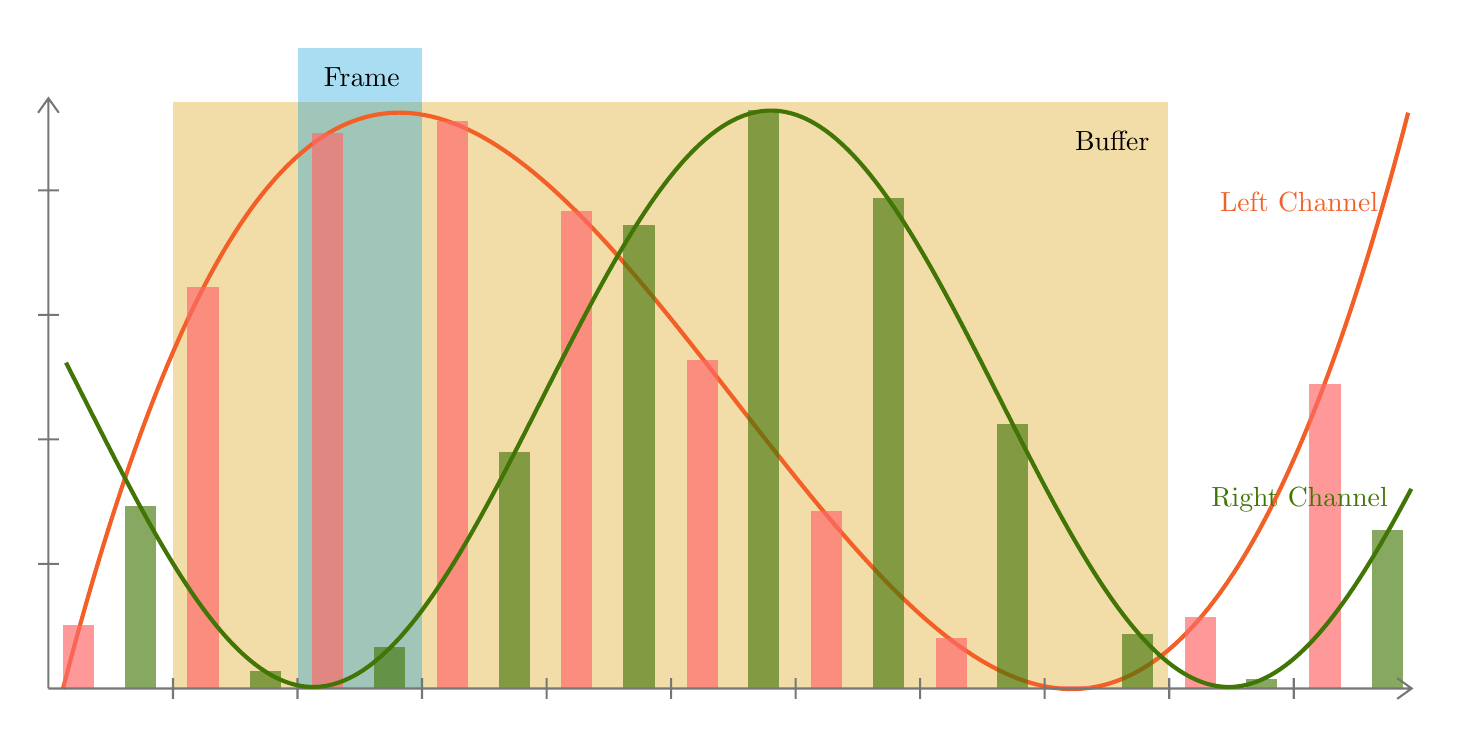
\begin{tikzpicture}[x=0.75, y=0.75,yscale=-1,xscale=1]
%\path (0,309); %set diagram left start at 0, and has height of 309
\clip (-10,-10) rectangle (667,319);

%Shape: Rectangle [id:dp8929919750163289] 
\draw  [draw opacity=0][fill={rgb, 255:red, 217; green, 151; blue, 0 }  ,fill opacity=0.34 ] (60,26) -- (539.33,26) -- (539.33,308.7) -- (60,308.7) -- cycle ;
%Shape: Rectangle [id:dp3527193498597476] 
\draw  [draw opacity=0][fill={rgb, 255:red, 0; green, 156; blue, 217 }  ,fill opacity=0.34 ] (120.32,0) -- (179.92,0) -- (179.92,308.37) -- (120.32,308.37) -- cycle ;
%Shape: Polynomial [id:dp29246577559714826] 
\draw  [color={rgb, 255:red, 242; green, 96; blue, 40 }  ,draw opacity=1 ][line width=1.5]  (6.97,308.65) .. controls (223.02,-524.46) and (439.07,864.05) .. (655.11,30.95) ;
%Shape: Rectangle [id:dp9419887277737906] 
\draw  [draw opacity=0][fill={rgb, 255:red, 255; green, 105; blue, 105 }  ,fill opacity=0.68 ] (6.97,277.71) -- (21.98,277.71) -- (21.98,308.37) -- (6.97,308.37) -- cycle ;
%Shape: Rectangle [id:dp5867675415467741] 
\draw  [draw opacity=0][fill={rgb, 255:red, 65; green, 117; blue, 5 }  ,fill opacity=0.63 ] (36.98,220.32) -- (51.98,220.32) -- (51.98,308.37) -- (36.98,308.37) -- cycle ;
%Shape: Rectangle [id:dp8838435632363444] 
\draw  [draw opacity=0][fill={rgb, 255:red, 255; green, 105; blue, 105 }  ,fill opacity=0.68 ] (66.99,114.8) -- (81.99,114.8) -- (81.99,308.37) -- (66.99,308.37) -- cycle ;
%Shape: Rectangle [id:dp9983336103528713] 
\draw  [draw opacity=0][fill={rgb, 255:red, 65; green, 117; blue, 5 }  ,fill opacity=0.63 ] (96.99,299.93) -- (112,299.93) -- (112,308.37) -- (96.99,308.37) -- cycle ;
%Shape: Rectangle [id:dp05075320113645709] 
\draw  [draw opacity=0][fill={rgb, 255:red, 255; green, 105; blue, 105 }  ,fill opacity=0.68 ] (127,40.74) -- (142,40.74) -- (142,308.37) -- (127,308.37) -- cycle ;
%Shape: Rectangle [id:dp7950673524144896] 
\draw  [draw opacity=0][fill={rgb, 255:red, 65; green, 117; blue, 5 }  ,fill opacity=0.63 ] (157.01,288.2) -- (172.01,288.2) -- (172.01,308.37) -- (157.01,308.37) -- cycle ;
%Shape: Rectangle [id:dp16650753615420033] 
\draw  [draw opacity=0][fill={rgb, 255:red, 255; green, 105; blue, 105 }  ,fill opacity=0.68 ] (187.01,35.19) -- (202.02,35.19) -- (202.02,308.37) -- (187.01,308.37) -- cycle ;
%Shape: Rectangle [id:dp5376486379245005] 
\draw  [draw opacity=0][fill={rgb, 255:red, 65; green, 117; blue, 5 }  ,fill opacity=0.63 ] (217.02,194.4) -- (232.02,194.4) -- (232.02,308.37) -- (217.02,308.37) -- cycle ;
%Shape: Rectangle [id:dp6362815105872923] 
\draw  [draw opacity=0][fill={rgb, 255:red, 255; green, 105; blue, 105 }  ,fill opacity=0.68 ] (247.03,78.39) -- (262.03,78.39) -- (262.03,308.37) -- (247.03,308.37) -- cycle ;
%Shape: Rectangle [id:dp2297523847438998] 
\draw  [draw opacity=0][fill={rgb, 255:red, 65; green, 117; blue, 5 }  ,fill opacity=0.63 ] (277.03,85.17) -- (292.04,85.17) -- (292.04,308.37) -- (277.03,308.37) -- cycle ;
%Shape: Rectangle [id:dp5777266331397943] 
\draw  [draw opacity=0][fill={rgb, 255:red, 255; green, 105; blue, 105 }  ,fill opacity=0.68 ] (307.5,149.97) -- (322.5,149.97) -- (322.5,308.37) -- (307.5,308.37) -- cycle ;
%Shape: Rectangle [id:dp8489472129971865] 
\draw  [draw opacity=0][fill={rgb, 255:red, 65; green, 117; blue, 5 }  ,fill opacity=0.63 ] (337.05,29.63) -- (352.05,29.63) -- (352.05,308.37) -- (337.05,308.37) -- cycle ;
%Shape: Rectangle [id:dp6863988849705387] 
\draw  [draw opacity=0][fill={rgb, 255:red, 255; green, 105; blue, 105 }  ,fill opacity=0.68 ] (367.51,222.79) -- (382.52,222.79) -- (382.52,308.37) -- (367.51,308.37) -- cycle ;
%Shape: Rectangle [id:dp35691755278546444] 
\draw  [draw opacity=0][fill={rgb, 255:red, 65; green, 117; blue, 5 }  ,fill opacity=0.63 ] (397.06,72.21) -- (412.06,72.21) -- (412.06,308.37) -- (397.06,308.37) -- cycle ;
%Shape: Rectangle [id:dp96707114333435] 
\draw  [draw opacity=0][fill={rgb, 255:red, 255; green, 105; blue, 105 }  ,fill opacity=0.68 ] (427.53,283.88) -- (442.53,283.88) -- (442.53,308.37) -- (427.53,308.37) -- cycle ;
%Shape: Rectangle [id:dp18768129092740105] 
\draw  [draw opacity=0][fill={rgb, 255:red, 65; green, 117; blue, 5 }  ,fill opacity=0.63 ] (457.07,180.83) -- (472.08,180.83) -- (472.08,308.37) -- (457.07,308.37) -- cycle ;
%Shape: Rectangle [id:dp620669459111896] 
\draw  [draw opacity=0][fill={rgb, 255:red, 255; green, 105; blue, 105 }  ,fill opacity=0.68 ] (487.54,307.33) -- (502.54,307.33) -- (502.54,308.37) -- (487.54,308.37) -- cycle ;
%Shape: Rectangle [id:dp3175842001170317] 
\draw  [draw opacity=0][fill={rgb, 255:red, 65; green, 117; blue, 5 }  ,fill opacity=0.63 ] (517.08,282.03) -- (532.09,282.03) -- (532.09,308.37) -- (517.08,308.37) -- cycle ;
%Shape: Rectangle [id:dp775060734049188] 
\draw  [draw opacity=0][fill={rgb, 255:red, 255; green, 105; blue, 105 }  ,fill opacity=0.68 ] (547.55,274.01) -- (562.56,274.01) -- (562.56,308.37) -- (547.55,308.37) -- cycle ;
%Shape: Rectangle [id:dp7574954211175227] 
\draw  [draw opacity=0][fill={rgb, 255:red, 65; green, 117; blue, 5 }  ,fill opacity=0.63 ] (577.1,303.63) -- (592.1,303.63) -- (592.1,308.37) -- (577.1,308.37) -- cycle ;
%Shape: Rectangle [id:dp4223776029333641] 
\draw  [draw opacity=0][fill={rgb, 255:red, 255; green, 105; blue, 105 }  ,fill opacity=0.68 ] (607.57,161.7) -- (622.57,161.7) -- (622.57,308.37) -- (607.57,308.37) -- cycle ;
%Shape: Rectangle [id:dp12596067869619243] 
\draw  [draw opacity=0][fill={rgb, 255:red, 65; green, 117; blue, 5 }  ,fill opacity=0.63 ] (637.78,232.05) -- (652.78,232.05) -- (652.78,308.37) -- (637.78,308.37) -- cycle ;
%Shape: Axis 2D [id:dp048941842347560494] 
\draw [color={rgb, 255:red, 118; green, 118; blue, 118 }  ,draw opacity=1 ][line width=0.75]  (0,308.37) -- (656.82,308.37)(0,24) -- (0,308.37) -- cycle (649.82,303.37) -- (656.82,308.37) -- (649.82,313.37) (-5,31) -- (0,24) -- (5,31) (60,303.37) -- (60,313.37)(120,303.37) -- (120,313.37)(180,303.37) -- (180,313.37)(240,303.37) -- (240,313.37)(300,303.37) -- (300,313.37)(360,303.37) -- (360,313.37)(420,303.37) -- (420,313.37)(480,303.37) -- (480,313.37)(540,303.37) -- (540,313.37)(600,303.37) -- (600,313.37)(-5,248.37) -- (5,248.37)(-5,188.37) -- (5,188.37)(-5,128.37) -- (5,128.37)(-5,68.37) -- (5,68.37) ;
\draw   ;
%Shape: Wave [id:dp3056897575840696] 
\draw  [color={rgb, 255:red, 65; green, 117; blue, 5 }  ,draw opacity=1 ][line width=1.5]  (8.47,151.39) .. controls (11.41,157.15) and (14.35,162.96) .. (17.3,168.79) .. controls (53.26,239.92) and (87.66,307.64) .. (127.57,307.64) .. controls (167.48,307.64) and (201.88,239.92) .. (237.84,168.79) .. controls (273.81,97.66) and (308.21,29.94) .. (348.12,29.94) .. controls (388.03,29.94) and (422.43,97.66) .. (458.39,168.79) .. controls (494.36,239.92) and (528.76,307.64) .. (568.67,307.64) .. controls (600.27,307.64) and (628.41,265.19) .. (656.62,212.2) ;

% Text Node
\draw (151,8) node [anchor=north] [inner sep=0.75pt]   [align=left] {Frame};
% Text Node
\draw (531.7,38.67) node [anchor=north east] [inner sep=0.75pt]   [align=left] {Buffer};
% Text Node
\draw (641.9,80) node [anchor=south east] [inner sep=0.75pt]   [align=left] {\textcolor[rgb]{0.95,0.38,0.16}{Left Channel}};
% Text Node
\draw (646.55,224.67) node [anchor=south east] [inner sep=0.75pt]  [color={rgb, 255:red, 65; green, 117; blue, 5 }  ,opacity=1 ] [align=left] {Right Channel};


\end{tikzpicture}
\end{document}